%% A simple template for a lab or course report using the Hagenberg setup
%% based on the standard LaTeX 'report' class
%% äöüÄÖÜß  <-- no German Umlauts here? Use an UTF-8 compatible editor!

%%% Magic comments for setting the correct parameters in compatible IDEs
% !TeX encoding = utf8
% !TeX program = pdflatex 
% !TeX spellcheck = en_US
% !BIB program = biber

\documentclass[english,notitlepage]{hgbreport}
\usepackage{pgfgantt}
\usepackage{array}
\newcounter{gantttask}
\newcounter{ganttsubtask}
\newcommand*{\alignmiddle}[2]{\multicolumn{1}{#1}{#2}}
\RequirePackage[utf8]{inputenc}		% remove when using lualatex oder xelatex!
\renewcommand{\chapter}[1]{}	% \chapter is deactivated
\renewcommand{\thesection}{\arabic{section}}
\setcounter{secnumdepth}{4}

\graphicspath{{images/}}   % where are the images?

\bibliography{references}   % requires file 'references.bib'
\ExecuteBibliographyOptions{backref=false}



%%-----------------------------------------------------------
\setcounter{chapter}{1}	% <----- set to assignment number!
%%-----------------------------------------------------------

\author{Gaurav Kumar Singh \\ \textit{\href{mailto:gauravks@mail.uni-paderborn.de}{gauravks@mail.uni-paderborn.de}}}
\title{Proposal for Master Thesis on topic \\
		Acceleration of Discontinuous Galerkin method \\
		using FPGAs communicating via IO channels}
\date{\today}


%%%----------------------------------------------------------
\begin{document}
%%%----------------------------------------------------------
\maketitle
%%%----------------------------------------------------------

\section{Introduction}

FPGA based accelerators provides the flexibility to design application specific hardware accelerators and re-use the same
hardware for different kinds of problems. Such advantages have shown an increased popularity of the FPGA accelerators among
the high performance computing (HPC) researchers in recent times. The FPGAs are mostly used to develop highly
optimized accelerators for common operations such as matrix multiplication, fast Fourier transformation
and sparse-matrix optimization which serve as the main computing blocks for many of the applications. These accelerators
mostly rely on the FPGA features such as pipelining for data re-use, replication for parallelization and memory localization
for lower memory latency.

The new Noctua high performance computing (HPC) cluster at Paderborn Center for Parallel Computing  (PC\textsuperscript{2})
which is equipped with additional Stratrix 10 FPGA accelerators provides an excellent opportunity to demonstrate the benefits
of using FPGA accelerators for applications from different domains. Along with the usual benefits mentioned previously, the
Nallatech 520N accelerator boards provides opportunities to use multiple FPGA in parallel for the same application by
using the four 100/40/25/10G QSFP28 network ports. These ports can be used to offload the network communication required in
some applications for data exchange via the MPI or similar distributed computing libraries. One such application
is MIDG2\footnote{\url{https://github.com/tcew/MIDG2}} which uses MPI to parallelize the computation on CPUs and GPUs.

MIDG2 is a MPI based parallel computation implementation of the Discontinuous Galerikin (DG) \cite{hesthaven_nodal_2008} method
to solve Maxwell's equation in time domain. DG method is a commonly used operation in many applications simulations to solve
partial differential equations (PDE). As it requires individual computation on the elements, many implementation
has been developed which are utilized by applications in different domains presented in \cite{ye_discontinuous_2011, wilcox_high-order_2010,
collis_discontinuous_2002}. There are other parallel implementation as well which utilize GPUs \cite{afzal_solving_2018, klockner_nodal_2009}
and multiple CPUs \cite{baggag_parallel_1999} for acceleration. \textcite{kenter_opencl-based_2018} presents an openCL based
FPGA accelerator which works for a single node and is 2x faster when compared to a multithreaded CPU implementation. Further acceleration
is possible using multiple FPGAs as shown by \textcite{kobayashi_opencl-ready_2018} where the authors compare the latency and bandwidth
of the communication between two FPGAs using FPGA-FPGA direct Ethernet communication and communication via CPU+InfiBand.
These implementation highlights the benefits of a FPGA based distributed computing system which is the main goal of this thesis.

In the rest of the document, the objectives of the thesis would be defined introducing some of the components involved followed
by the timeline and initial outline of the thesis work.


\section{Objectives}

The Noctua being first of the academic HPC cluster equipped with FPGAs, there is no known implementation
utilizing FPGA in network configuration for more than two FPGAs. The proposed master thesis aims at presenting
such a system which evaluates the achievable acceleration with multiple FPGAs using point-to-point communication
in different network topologies for the MIDG2 application. To reach the final aim following objectives are
required to be achieved as part of this thesis:

\begin{enumerate}
	\item \textbf{Objective 1}: Identify and evaluate possible topologies using the 4 IO channels on Nallatech 520N boards
	\item \textbf{Objective 2}: Extend the openCL kernels of the MIDG2 FPGA implementation to use IO channels
	\item \textbf{Objective 3}: Devise an effective partitioning scheme for the mesh to reduce communication overheads for the target topologies
\end{enumerate}

\subsection{Objective 1}

The current Nallatech BSP for 520N supports 4 openCL IO channels based communication between
multiple FPGA using the 100/40/25/10G QSFP28 network ports. The first objective of
the thesis is to utilize these network ports to evaluate and identify a point-to-point
topology for the FPGA which is most effective for the MIDG2 implementation.

\subsubsection{IO Channels}

The openCL IO channels provided by the BSP are an extension of the standard Intel channels \cite{noauthor_intel_2018}
and can be used in similar way to provide blocking communication between multiple FPGAs.
Current version of the IO channels supports a maximum data rate of 40 Gbits/s using 256 bits per cycle.
As there is no MAC mechanism available yet, only point-to-point communication is possible between
two FPGAs.

\subsubsection{Proposed Topologies}

To identify a suitable topology for the application, multiple topologies
as shown in figure \ref{fig:topologies} would be evaluated. The main criteria for the evaluation
would be latency and the overall bandwidth of the channels achieved in each
configuration. As the topology shall be known prior to execution of the application,
the topological information should be provided by a suitable topological file
to enable the FPGAs identify their neighbors.

\begin{figure}[h]
	\centering\small
	\begin{tabular}{c@{\hskip 0.5in}c}
		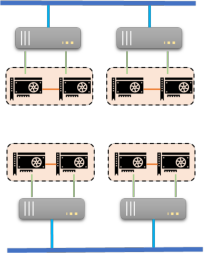
\includegraphics[width=0.35\textwidth]{topo1} &		% JPEG file
		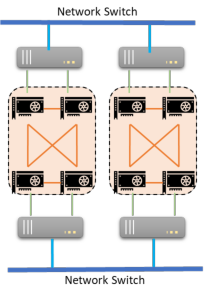
\includegraphics[width=0.35\textwidth]{topo2} \\	% PNG file
		(a) Within Node & (b) Fully connected no HOPS \\ \\
		\alignmiddle{m{0.35\textwidth}@{\hskip 0.5in}}{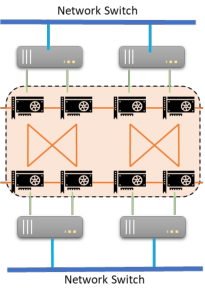
\includegraphics[width=0.35\textwidth]{topo3}} &		% JPEG file
		\alignmiddle{m{0.35\textwidth}}{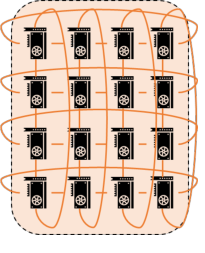
\includegraphics[width=0.35\textwidth]{topo4}} \\	% PNG file
		(c) Fully connected with HOPS & (d) Toroidal
	\end{tabular}
	\caption{Proposed topologies. (a), (b) and (d) are partially connected and (c) is
	fully connected topologies} 
	\label{fig:topologies}
\end{figure}

\subsection{Objective 2}

The second objective is to extend the MIDG2 FPGA implementation to use IO Channels for communicating
the shared elements information using the topologies identified in previous step.
This step requires understanding of following components.

\subsubsection{Nodal Discontinuous Galerikin Method}	% title of a subtask

The nodal discontinuous Galerikin time domain method (DGTD) \cite{hesthaven_nodal_2008} is used to find solutions
for partial differential equations (PDE) numerically. The method is proved to be efficient in
producing results with computers as it relies on mathematical calculations on elemental basis.
This allows to perform computation in parallel on similar or different hardware helping to
solve problems from different domains quickly. DGTD method is particularly popular for applications
in the domains such as fluid mechanics, plasma physics and electrodynamics.

\textcite{Hesthaven_190449} presents the use of DGTD to solve time-domain Maxwell's equations with an 1D example.
These equations serve as the base for solving many of the electrodynamics problems and is adopted by
many computer based algorithms as well. MIDG2 is once such implementation which uses K non-overlapping tetrahedra elements
for computing the fields value using Maxwell's equations. The original MIDG2 implementation supports
parallelization using MPI for multiple CPUs and uses OCCA \footnote{\url{https://libocca.org}} to provide
support for acceleration with GPU using CUDA and openCL. An extended version of MIDG2 which used openCL and
MPI to provide acceleration will be used as the reference design.

\subsubsection{MIDG2 MPI FPGA implementation}
MIDG2 MPI FPGA is extended version of MIDG2 application utilizing openCL kernels to perform the
computation and MPI for communication between multiple nodes. The openCL kernels are
highly optimized to achieve maximum performance on a single FPGA using pipelining using
standard Intel channels. This implementation will be used as the reference design and
the existing architecture of the application is shown in figure \ref{fig:kernels}.
The DG time domain computation are performed in time steps using multiple kernels.
Volume and the surface kernel are used to compute the volume and surface RHS field
contributions of the elements respectively. The RK kernel accumulates the RHS
field contribution computed in volume and surface kernel. Partial kernel reads in
the intermediate fields value of last time step from the FPGA memory and fills them
in a contiguous memory which is then distributed to the respective neighbors using
MPI asynchronous communication.

\begin{figure}[h]%
    \centering
    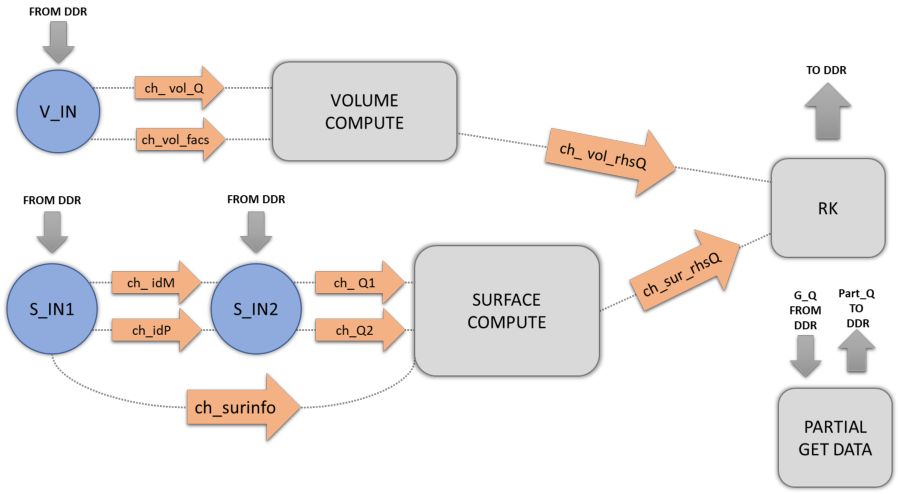
\includegraphics[width=1.0\textwidth]{images/kernels}
    \caption{openCL kernels for MIDG2 MPI FPGA implementation}
    \label{fig:kernels}
\end{figure}

In order to achieve communication between multiple FPGAs, IO channels would be used
in the partial kernel to send the data directly to the neighboring FPGA.

\subsection{Objective 3}

The third objective is to identify a suitable partitioning configuration for the mesh elements so that
the distribution of the elements among the FPGAs utilizes the topological information. This is critical
as a good distribution scheme would reduce the overall network communication by placing neighboring elements
on neighboring nodes. The partitioning is currently done by the ParMETIS\footnote{\url{http://glaros.dtc.umn.edu/gkhome/metis/parmetis/overview}}
library. 

\subsubsection{ParMETIS}

ParMETIS is a MPI-based parallel library which is capable of partitioning a variety of unstructured graphs and meshes. MIDG2
uses the ParMETIS to partition the mesh elements among the MPI nodes. The partitioning api uses a set of parameters such as element
size, partitioning surface criteria and weights for distribution considering capabilities of the node. These parameters allow
ParMETIS to partition the mesh into section which reduces the overall shared elements among nodes and reduce the communication requirement.
The partitioning scheme would require to be updated in order to provide the ParMETIS library the information of the topology of the FPGA.

\section{Preliminary Outline}
\begin{enumerate}
	\item Introduction
	\item Fundamentals and Related Work
	\begin{enumerate}
		\item Nodal Galerikin Discontinuous method
		\item Fundamental of openCL
		\item IO channels
	\end{enumerate}
	\item System Architecture of updated design
	\begin{enumerate}
		\item Topology configurations
		\item openCL kernel structure
		\item Host application updates
	\end{enumerate}
	\item Evaluation
	\begin{enumerate}
		\item Comparision of topologies
		\item Comparision with reference design
	\end{enumerate}
	\item Conclusion

\end{enumerate}

\section{Proposed Time Schedule}


\begin{ganttchart}[
	vgrid,
	bar label node/.append style={text width=4cm},
	group label node/.append style={text width=4cm},
	bar label text={\refstepcounter{ganttsubtask}\arabic{gantttask}.\arabic{ganttsubtask} \strut#1},
	group label text={\setcounter{ganttsubtask}{0}\refstepcounter{gantttask}\arabic{gantttask}. \strut#1},
	]{1}{24}
    \ganttset{bar height=.25}
    \gantttitle{Master's Thesis Timeline - Week Numbers}{24} \\
    \gantttitlelist{44,...,52}{1}
    \gantttitlelist{1,...,15}{1} \\

    \ganttgroup{Prototype kernels to test IO Channels}{1}{5} \\
	\ganttbar{basic IO channel communication}{1}{2} \\
	\ganttbar{prototype for\\ selected topologies}{3}{5} \\

	\ganttgroup{MIDG2 application Update}{6}{15} \\
    \ganttbar{update kernel with IO channel}{6}{8} \\
    \ganttbar{implement for 2 FPGA}{9}{10} \\
    \ganttbar{update for multiple FPGA}{11}{13} \\
    \ganttbar{devise partitioning scheme}{14}{15} \\

    \ganttgroup{Evaluation}{16}{19} \\
    \ganttbar{add evaluation code}{16}{16} \\
    \ganttbar{test different topologies}{17}{18} \\
    \ganttbar{consolidate results}{19}{19} \\

    \ganttgroup{Final report}{20}{22} \\
    
    % \ganttmilestone{review}{36} \ganttnewline
\end{ganttchart}

The time plan is scheduled considering 22 weeks of work time starting from 1st of November 2018.
Approach is to first prototype the topological evaluation to identify possibilities and test them,
followed by implementation of the changes required in the MIDG2 MPI FPGA application to support
multiple FPGA using IO channels. In the last a detailed evaluation and final thesis preparation is
planned.
%%%----------------------------------------------------------

\pagebreak
\section*{References}

\printbibliography[heading=noheader]

%%%----------------------------------------------------------

\end{document}
